\subsection{Tiling}

\frame{
  \frametitle{Representing Collision Strings}

  \begin{itemize}
    \item Reflect squares about each side to create a tiling
    \item Solutions become lines in the plane
    \item Intersections become places where collisions occur
  \end{itemize}
}

\frame{
  \frametitle{Representing Collision Strings}

  \begin{example}
    Tiling of $\vec{x}_0 = (0, 0.5)$ and $\vec{v} = (0.25, 0.25)$.
  \end{example}

  \begin{columns}
    \begin{column}{0.45\textwidth}
      \begin{figure}
        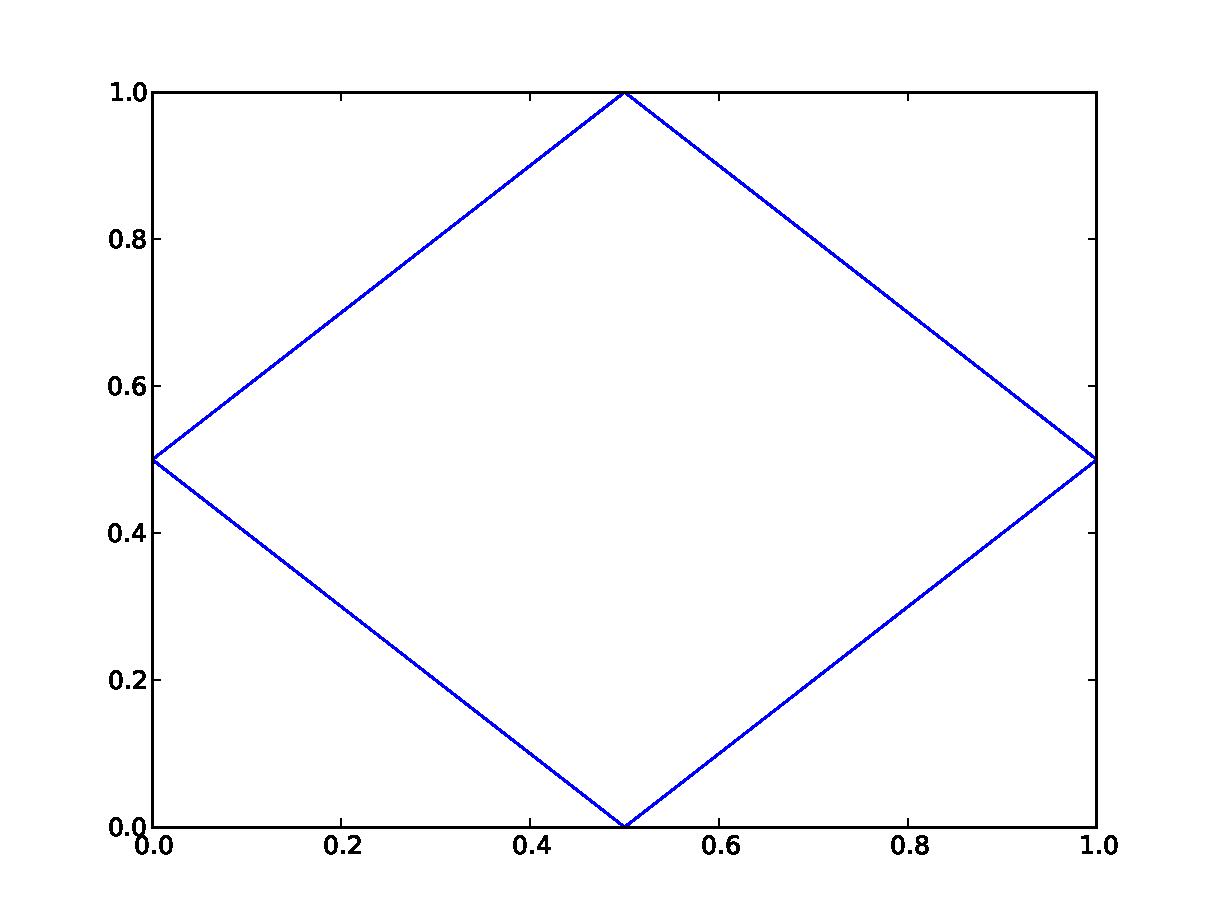
\includegraphics[width=2.1in]{abab.pdf}
      \end{figure}
    \end{column}
    \begin{column}{0.45\textwidth}
      \begin{figure}
        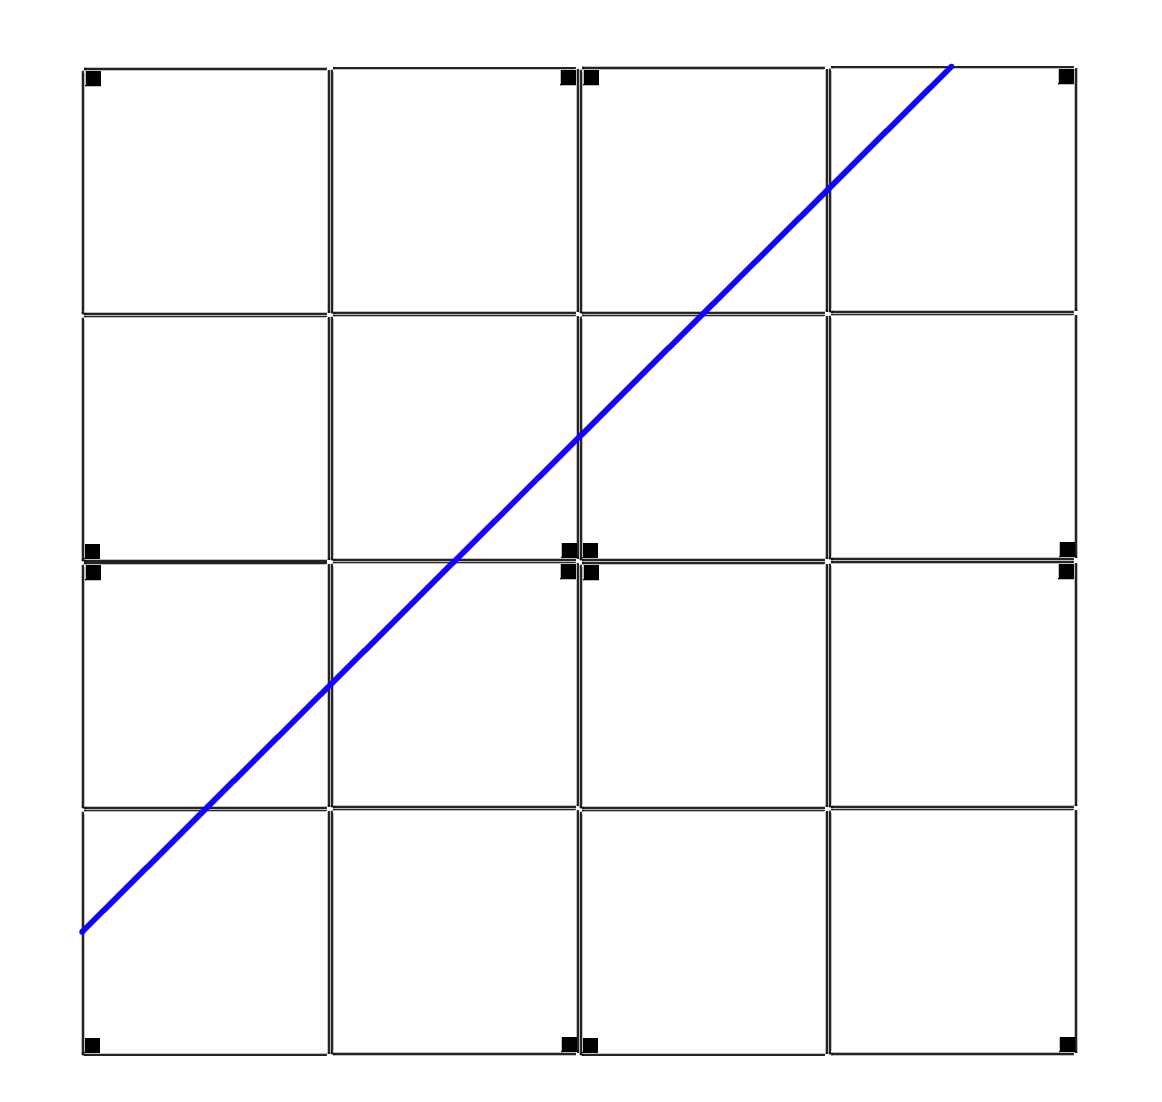
\includegraphics[width=1.7in]{tiling.png}
      \end{figure}
    \end{column}
  \end{columns}
}
